\documentclass{article}

\usepackage{arxiv}

%%% Columns
\usepackage{multicol}

%%% Polices et langue
\usepackage[hyphens]{url}         % Pour citer les adresses web
\usepackage{hyperref}             % Citations plus complètes
\usepackage[T1]{fontenc}          % Encodage des accents
\usepackage[utf8]{inputenc}       % Lui aussi

%%% Couleurs et modification sur l'écriture
\usepackage[svgnames]{xcolor}     % De la couleur
\usepackage{cancel}               % Pour les traits
% \usepackage[margin=2cm]{geometry} % Gérer correctement la taille
\usepackage{enumitem}

%%% Symboles mathématiques
\usepackage{amsmath}              % La base pour les maths
\usepackage{mathrsfs}             % Quelques symboles supplémentaires
\usepackage{amssymb}              % encore des symboles.
\usepackage{amsfonts}             % Des fonts, eg pour \mathbb.

%%% Pour les dessins, les graphiques, ...
\usepackage{stackengine}
\usepackage{float}
\usepackage{graphicx}             % inclusion des graphiques
\usepackage{caption}
\usepackage{subcaption}
\usepackage{wrapfig}              % Dessins dans le texte
\usepackage{array}                % Pour avoir des colonnes personnalisées
\newcolumntype{P}[1]{>{\centering\arraybackslash}p{#1}} % Colonne centrée
\usepackage{makecell}             % Allow for intricated tables

%%% Pour représenter les algorithmes
\usepackage[noend, ruled, french, onelanguage]{algorithm2e}

%%% Special commands

% Uncomment to remove the header
\pagestyle{plain}

% Uncomment to override  the `A preprint' in the header
\renewcommand{\headeright}{}
\renewcommand{\undertitle}{}
% \renewcommand{\shorttitle}{\textit{arXiv} Template}

% Les guillemets \ofg{par exemple}
\newcommand{\ofg}[1]{\og{}#1\fg{}}
% Des parenthèses, crochets et accolades qui s'adaptent automatiquement à
% la taille de ce qu'il y a dedans
\newcommand{\pa}[1]{\left(#1\right)}
\newcommand{\pac}[1]{\left[#1\right]}
\newcommand{\paa}[1]{\left\{#1\right\}}
% Pour faire des indices en mode texte
\newcommand{\e}[1]{_{\text{#1}}}
% Pour avoir une couleur uniquement sur les traits
\newcommand{\Cancel}[2][black]{{\color{#1}\cancel{\color{black}#2}}}

% Customized bibliography
\let\OLDthebibliography\thebibliography
\renewcommand\thebibliography[1]{
  \OLDthebibliography{#1}
  \setlength{\parskip}{0pt}
  \setlength{\itemsep}{0pt plus 0.3ex}
}

% For having figures in the two-column environment
\newenvironment{Figure}
  {\par\medskip\noindent\minipage{\linewidth}}
  {\endminipage\par\medskip}

%%% Title

% Mettez votre titre et votre nom ci-après
\title{Summary Source Prediction}
\author{
  \textbf{Sébastien Meyer} \\
  École polytechnique, France \\
  \texttt{sebastien.meyer@polytechnique.edu}
}
% À décommenter si vous ne voulez pas que la date apparaisse explicitement
\date{}

%%% The document itself

\begin{document}

\maketitle

\begin{multicols}{2}

  This report details the different approaches and strategies that I have developed in order
  to get the best possible score I could on the summary source data set. We were given a
dataset made up of a
gathering of original documents as well as their summary, either human-written or generated by a machine. There were also additional documents. The main task was to predict whether the summary was generated by a machine or not. We had
a training set and we were asked to submit a csv file containing a label associated
to each
summary.

It has
been a really challenging project for me. In order
to best describe how I tackled this problem, this report will follow my advances. Firstly, I
will remind the reader with a brief description of the task and the data. Then, I will go on
with my first attempts. Since my first tries were not satisfactory,
I took inspiration from past projects to get
new ideas. In the 
\textbf{Appendix}, I gathered my models with some details on the
pipeline.

\section{The dataset}

The dataset is made up of 8000 training points and 3200 test points. It appears that the
training
set is not very large. Therefore, we
must be prepared to face overfitting. Our task is a classification task, corresponding to
the \textit{label} variable, which is binary. The training set is perfectly balanced, as each class accounts for
4000 of the 8000 samples (see \textbf{Figure \ref{fig:labelrepart}}).

\begin{Figure}
    \centering
    \captionsetup{type=figure}
    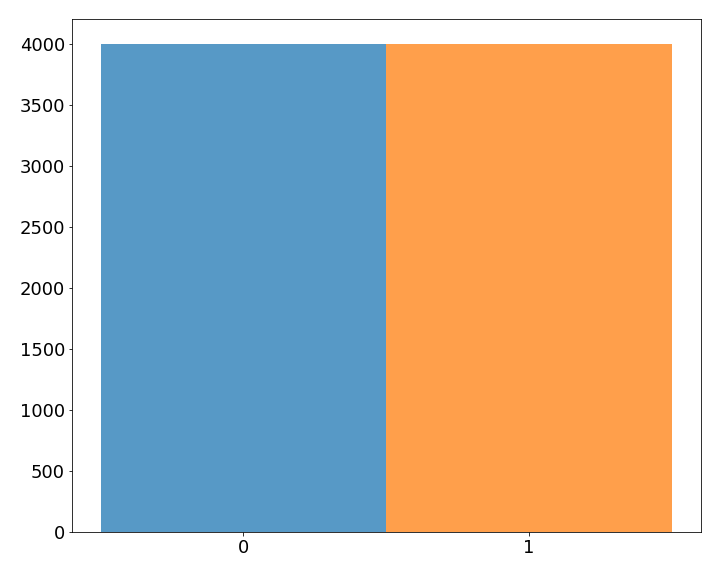
\includegraphics[width=0.7\linewidth]{figures/label_repart.png}
    \captionof{figure}{Repartition of the training labels.}
    \label{fig:labelrepart}
\end{Figure}

For each sample, we recognize a document, which is the original document from which the summary is created, and the corresponding summary. Some basic information about the training documents and summaries are gathered in \textbf{Table \ref{tab:featsum}}. We also show an example of summary associated with label 0 and another one associated with label 1 in \textbf{Figure \ref{fig:twoex}}. We can directly observe that there are some differences between the two summaries. Indeed, the first summary lacks coherence between its two sentences. Also, there are a lot of spaces and special characters in the summary. On the contrary, the second summary is associated to label 0 and seems pretty clear and well-written. There is a clear correspondance between words, verbs and pronouns.

\begin{center}
\captionsetup{type=tabular}
  \begin{tabular}{|c|cccc|}
    \hline
    Feature & Mean & Std & Min. & Max. \\
    \hline
    Doc. len. & 3.974 & 2,052 & 297.0 & 12,052 \\
    Sum. len. (0) & 304.6 & 78.91 & 68.0 & 675.0 \\
    Sum. len. (1) & 308.0 & 134.3 & 64.0 & 3,524 \\
    \hline
  \end{tabular}
\captionof{table}{Description of numerical variables.}
\label{tab:featsum}
\end{center}

\begin{Figure}
  \centering
  \captionsetup{type=figure}
  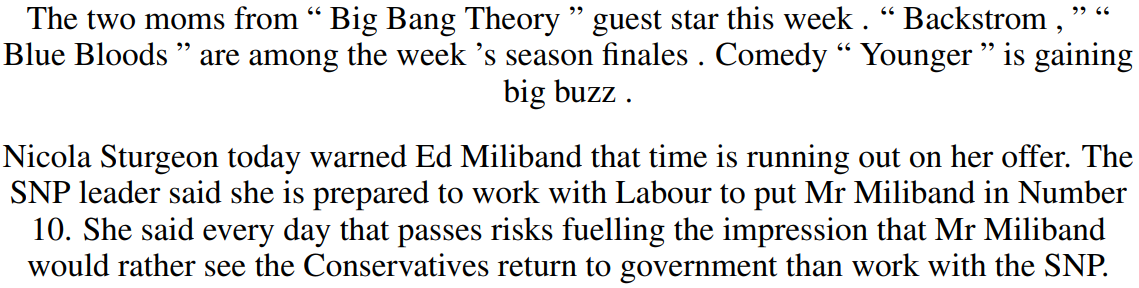
\includegraphics[width=\linewidth]{figures/two_examples.png}
  \captionof{figure}{First summary has label 1, second has label 0.}
  \label{fig:twoex}
\end{Figure}

These observations led me to create some features from the documents and summaries. Recall that our features are gathered in the \textit{src/preprocessing/features} folder. I computed different features under the name \textit{X\_Y} where \textit{Y} can be \textit{count} for the number of observed instances, \textit{ratio} for the ratio between the values of \textit{count} for the summary and the document and \textit{overlap}. The \textit{overlap} is defined as follows: all items are selected and put into a set, the intersection of the set of the document and the set of the summary is computed and its length is the value associated to the feature. The first feature for this case is \textit{char\_Y} for the total length of the text. In addition, I computed similar features for words under \textit{word\_Y}, for sentences under \textit{sent\_Y} and for groups of consecutive words beginning with an upper letter under \textit{group\_Y}. On top of that, I added some minor features such as \textit{upper\_char}, \textit{upper\_word}, \textit{numeric} and \textit{dash} which address special characters, as well as \textit{is\_first\_upper} and \textit{is\_last\_ponct} to look at specificities. 

\section{First attempts}

My first models are based on the features presented in the previous section as well as tf-idf features. The baseline logistic regression with 10,000 tf-idf features yields an accuracy of approx. 0.62 on the test set. Therefore, there is much room more improvement. Also, since I started working with binary and categorical variables, I decided to work with trees. Let $X$ be a feature gathering
binary variables and thus having values from 1 to $p$. When splitting
at a specific node,
a decision tree can make a decision based on $X > a$ or $X \leq a$.
We see that such decision implies that values between 1 and $a$ have
a relationship, which is the case for a lot of features that we computed.

\subsection{Cross-validated gridsearch}

I implemented an automated gridsearch pipeline
using \textit{optuna} package to select the parameters of any model
I decided to use. \textit{Optuna}\cite{optuna} takes ranges of values for
model parameters as entry, and performs an optimization to find the best
parameters according to the cross-validation score. The cross-validation
was 5 folds large, with accuracy as target. Typically, I would run a
gridsearch for 15 to 50 trials, depending on the complexity of the model
and the size of the dataset. This would not take much more than 30 minutes.

\subsection{RandomForestClassifier, ExtraTreesClassifier and LightGBM}

The first models that I used were RandomForestClassifier and ExtraTreesClassifier from \textit{scikit-learn}\cite{sklearn} API. These models are widely used in the case of classifications with more
than two possible labels. For instance, RandomForestClassifier relies on
the averaging of several base decision trees. These decision
trees are built in a top-bottom fashion. Each split builds two nodes or
regions $R$ and $\bar{R}$. Let us denote by $p^{R}_k$ and $p^{\bar{R}}_k$
the proportions of samples from class $k$ falling respectively in regions
$R$ and $\bar{R}$. Split is made by minimizing a criterion, the most used
criterion being Gini index defined as:

\begin{center}
  $$
  C(R, \bar{R}) = \sum \limits_{k} p^R_k (1 - p^R_k) +
  \sum \limits_{k} p^{\bar{R}}_k (1 - p^{\bar{R}}_k)
  $$
\end{center}

\noindent which is the sum of Gini impurities in both $R$ and $\bar{R}$.
Other criterions can be used and have been tried during gridsearch, namely entropy
criterion, however Gini index yields best results in almost all runs. ExtraTreesClassifier is
based on trees that differ from usual decision trees in two points:

\begin{enumerate}[wide, labelindent=5pt, itemsep=0pt, topsep=0pt]
  \item Bootstrapping is disabled by default for ExtraTreesClassifier
  \item Splits are chosen among randomly drawn cuts given a subset of features
\end{enumerate}

In some cases, such extremely randomized decisions can reduce overfitting,
but it does not appear to be the case for our data set. Later, I started using boosting models such as LightGBM\cite{lightgbm}. Although LightGBM is based
on the same principle as other boosting models, that is, updating a model by
successively assigning weights to wrongly classified data points, it is designed to
be much more faster on large datasets than its counterparts.

A basic
gridsearch for RandomForestClassifier
lead to an accuracy of 0.8206, other models having lower scores. This score
was relatively good, considering that I did not start extensive feature engineering
and that my models were rather simple. However, tweaking these models did not bring much
improvement. I had to start engineering new features.

\subsection{Stacking}

Even though RandomForestClassifier appears to outperform other models, Boosting
models such as LightGBM and XGBoost\cite{xgboost} perform relatively well on
the dataset and yield similar results to RandomForestClassifier. One of the methods
used to combine different models that can be good at predicting specific aspects
of the data is through Stacking. In the \textit{scikit-learn} API, several base
models are fitted
on the training dataset. Then, a final estimator - usually a LogisticRegression -
is fitted on base estimators predictions over training data with cross-validation
to avoid overfitting. A summary schema is shown \textbf{Figure \ref{fig:stacking}}.
In this model, I tried to combine different models such as
RandomForestClassifier, XGBoost and LightGBM. 

\begin{Figure}
  \centering
  \captionsetup{type=figure}
  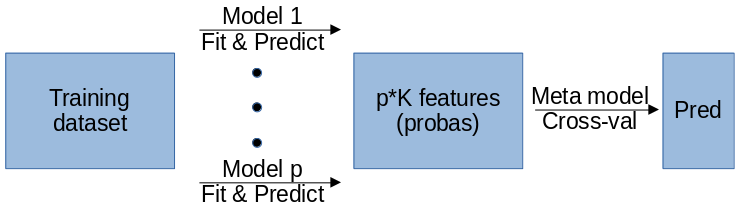
\includegraphics[width=0.75\linewidth]{figures/stacking_schema.png}
  \captionof{figure}{Stacking pipeline.}
  \label{fig:stacking}
\end{Figure}

Since Stacking uses several models, its training is much more longer than for
any base estimator. Therefore, running a gridsearch for the Stacking model would
be computationally too expensive for my computer. I decided to fix the parameters
of the base estimators using the best parameters of their own gridsearch.

\section{Taking inspiration from past projects}

\subsection{New features}

Until now, I generally separated the features either from regex expression or from tf-idf decomposition. A simple improvement to my results came from the concatenation of these features. In order not to have 10,000 tf-idf features against around 10 regex features, I performed truncated Singular Value Decomposition, which approximates a PCA for sparse matrices such that the ones we get from tf-idf decomposition using \textit{scikit-learn} API. Moreover, I implemented a composition function to allow us to compute normalizations\cite{tfidfcomp} of tf matrices. However, the different compositions did not bring much improvement in regard to the natural term-frequency matrices. In addition, I computed the cosine similarity between the summary and its original document as a new feature. Together with an ExtraTreesClassifier model, I was able to reach an accuracy of 0.84937. 

Nevertheless, a major breakthrough originated from a very simple feature. Indeed, I computed a feature which counts the number of spaces before a ponctuation using a regex expression. As shown \textbf{Figure \ref{fig:spacbef}}, almost none of the generated summaries present spaces before ponctuation. Therefore, this feature helped us reach a new highscore. In a Stacking model including RandomForestClassifier, LightGBM, XGBoost and ExtraTreesClassifier, I reached an accuracy of 0.89937.

Other improvements came from minor features. For instance, recall that sentences can be transformed into Part-of-Speech tagging. In this case, each token is associated with a tag which must describe its role in the text, for example noun or adjective. I used all the available tags in \textit{nltk} package and computed lots of features, again with \textit{count}, \textit{ratio} and/or \textit{overlap} versions. These new features with a Stacking model allowed me to reach an accuracy of 0.90625.

Another type of features which I looked into is latent semantic analysis. The \textit{scikit-learn} package offers different ways of performing latent semantic analysis. In one case, Latent Dirichlet Allocation or LDA allows to find important topics in a corpus, thanks to tf-idf decomposition. I manually computed the 3 most important topics and used some or all of them as features. This allowed me to reach an accuracy of 0.91312, using LightGBM. In fact, LightGBM started to show better results than Stacking when sufficiently extensive grid search was performed. 

Finally, I found GLTR\cite{gltr}. This model is based on existing models, for instance BERT and GPT-2, and uses them to predict whether if words in a sentence were likely to be generated by this type of models. I used the estimated probabilities for all the words in a summary to compute bins of fractions of probabilities and of topk values. With LightGBM model, I reached an accuracy of 0.91875.

\begin{Figure}
  \centering
  \captionsetup{type=figure}
  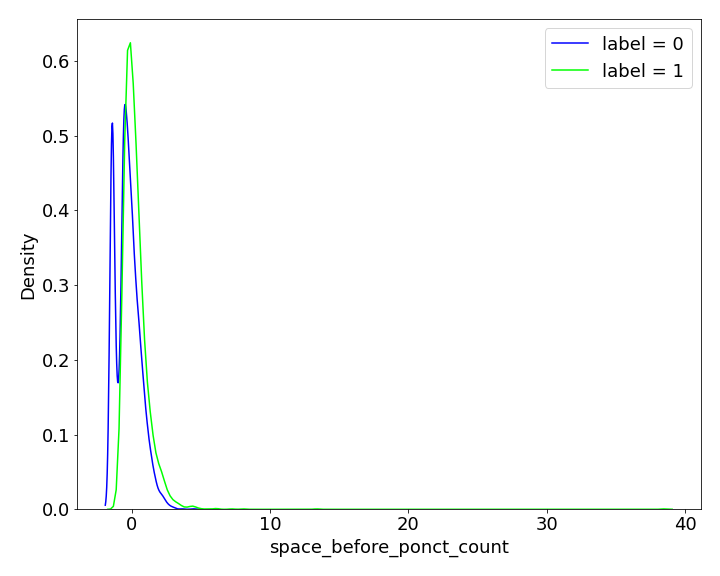
\includegraphics[width=0.75\linewidth]{figures/space_before_ponct_count_repart.png}
  \captionof{figure}{Repartition of training labels wrt \textit{space\_before\_ponct\_count}.}
  \label{fig:spacbef}
\end{Figure}

\section{Last improvements}

\subsection{Failed attempts}

There are two major paths that did not lead me to good results. On the one hand, I tried to use embeddings. I performed the usual tokenization and padding of the summaries, and I used either the GloVe\cite{glove}, GoogleNews\cite{word2vec} available embeddings, or I trained my own Word2Vec vocabulary and embeddings using \textit{gensim}. Then, I used different neural networks, from feed-forward to bidirectional LSTMs. However, I was not able to go over an accuracy of 0.68 in a train-test-split setting. 

On the other hand, recall that very powerful models for text generation already exist. Also, my recent findings on GLTR made me think that I could use existing models for detecting generated summaries. To that extent, I used the huggingface\footnote{https://huggingface.co/} library in order to find models shared by the community. Here, I faced two major issues. Firstly, most of the models are not fitting on my GPU, which is capped at 6GB. Secondly, there were not a lot of available models that were built for our classification task. I tried with some models such as DistilBERT and DistilroBERTa. After some epochs, it is possible to achieve competitive results, however, I did not continue with these models.

\subsection{Feature selection and Catboost}

My last improvements come from the \textit{mlxtend}\cite{mlxtend} package, which offers sequential feature selector. I also tried other well-known models, namely CatBoost\cite{catboost}. CatBoost is a boosting model particularly adapted to categorical features. My final accuracy is 0.92812. Similar feature selection with a Stacking model gathering RandomForestClassifier, XGBoost, LightGBM and CatBoost brings me to an accuracy of 0.92187, which is not more than the one achieved with CatBoost alone.

\section*{Conclusion}

To conclude, I have learnt some practical skills from this project. 
Most of the time, it is difficult to get a precise idea of a model or 
even a pipeline to address a dataset. One has to try and search different 
combinations. All in all, we can keep in mind that once a baseline is found by 
using an usual model, other less "conventional" models can be tested out. 
In terms of the competition itself, one of the most important aspects was to 
design pertinent features. This challenge allowed me to learn more about 
data analysis ideas and to be more careful about the models we use on a regular 
basis. Despite my satisfactory results, I think 
that things can still be done to improve my models. If I had more time, I
would have tried to build more features, especially from the semantic analysis which remained mysterious to me. In addition, more computational power would 
allow for more aggressive gridsearch and the use of other huggingface models!


%% Bibliographie intégrée (personnalisable)

\begin{thebibliography}{9}

\bibitem{optuna}
Takuya Akiba, Shotaro Sano, Toshihiko Yanase, Takeru Ohta and Masanori Koyama.
\textit{Optuna: A Next-generation Hyperparameter Optimization Framework.} 2019, in KDD.

\bibitem{lightgbm}
Guolin Ke, Qi Meng, Thomas Finley, Taifeng Wang, Wei Chen, Weidong Ma, Qiwei Ye and Tie-Yan Liu.
\textit{LightGBM: A Highly Efficient Gradient Boosting Decision Tree.} Advances in Neural
Information Processing Systems 30 (NIPS 2017), pp. 3149-3157.

\bibitem{sklearn}
F. Pedregosa, G. Varoquaux, A. Gramfort, V. Michel, B. Thirion, O. Grisel, M. Blondel,
P. Prettenhofer, R. Weiss, V. Dubourg, J. Vanderplas, A. Passos, D. Cournapeau, M. Brucher,
M. Perrot and E. Duchesnay. \textit{Scikit-learn: Machine Learning in Python.} 2011. Journal
of Machine Learning Research, vol.12, pp. 2825-2830.

\bibitem{xgboost}
Tianqi Chen and Carlos Guestrin. \textit{XGBoost: A Scalable Tree Boosting System.}
San Francisco, California, USA. 2016. Proceedings of the 22nd ACM SIGKDD International
Conference on Knowledge Discovery and Data Mining, pp. 785-794.

\bibitem{tfidfcomp}
François Rousseau and Michalis Vazirgiannis. \textit{Composition of TF Normalizations: New Insights on Scoring Functions for Ad Hoc IR.} ACM, SIGIR 2013.

\bibitem{gltr}
Sebastian Gehrmann, Hendrik Strobelt and Alexander M. Rush. \textit{GLTR: Statistical Detection and Visualization of Generated Text.} June 2019. (Available at: https://arxiv.org/pdf/1906.04043.pdf)

\bibitem{glove}
Jeffrey Pennington, Richard Socher and Christopher D. Manning. \textit{GloVe: Global Vectors for Word Representation.} 2014.

\bibitem{word2vec}
Tomas Mikolov, Kai Chen, Greg Corrado and Jeffrey Dean. \textit{Efficient Estimation of Word Representations in Vector Space.} Septembre 2013. (Available at: https://arxiv.org/pdf/1301.3781.pdf)

\bibitem{mlxtend}
Sebastian Raschka. \textit{MLxtend: Providing machine learning and data science utilities and extensions to Python's scientific computing stack.} 2018. J Open Source Softw 3 (24). 

\bibitem{catboost}
Anna Veronika Dorogush, Vasily Ershov and Andrey Gullin. \textit{CatBoost: gradient boosting with categorical features support.} Workshop on ML Systems at NIPS 2017.

\end{thebibliography}

\end{multicols}

\newpage

\section*{Appendix}

\subsection*{Models and results}

The following tables sum up the different submissions we made as well as corresponding
features and tuned parameters. All runs and gridsearches were made with at least one of
the following
seeds: 42, 1342 and 8005.

\begin{table}[H]
\centering
\resizebox{\columnwidth}{!}{%
\begin{tabular}{|c||c|c|c||c|}
  \hline
  Model & Preprocessing & Features & Tuned Parameters & Test accuracy \\
  \hline
  \hline
    RandomForestClassifier &
    \makecell{
      Eliminate correlated var.: No \\
      PCA: No \\
      Scaling: Standard} &
    \makecell{
      \textit{char\_X} + \textit{word\_X} + \textit{sent\_X} \\
      + \textit{upper\_char\_X} + \textit{upper\_word\_X}  \\
      + \textit{numeric\_X} + \textit{dash\_X} + \textit{group\_X} \\
      + \textit{is\_first\_upper} + \textit{is\_last\_ponct} \\
      \textbf{Total: 26}} &
    \makecell{
      \textit{n\_estimators} \\
      \textit{criterion} \\
      \textit{max\_depth} \\
      \textit{min\_samples\_split} \\
      \textit{min\_samples\_leaf} \\
      \textit{max\_features} \\
      \textit{ccp\_alpha}} &
    0.82062 \\
  \hline
    ExtraTreesClassifier &
    \makecell{
      Eliminate correlated var.: No \\
      PCA: No \\
      Scaling: Standard} &
    \makecell{
      previous \\
      + \textit{n\_idf\_cos} + \textit{n\_idf\_pca\_1} \\
      \textbf{Total: 28}} &
    \makecell{
      \textit{n\_estimators} \\
      \textit{criterion} \\
      \textit{min\_samples\_split} \\
      \textit{min\_samples\_leaf} \\
      \textit{max\_features} \\
      \textit{min\_impurity\_decrease} \\
      \textit{ccp\_alpha}} &
    0.84937 \\
  \hline
  \makecell{
    Stacking: \\
    - RandomForestClassifier \\
    - ExtraTreesClassifier \\
    - XGBoost \\
    - LightGBM} &
  \makecell{
    Eliminate correlated var.: No \\
    PCA: No \\
    Scaling: Standard} &
  \makecell{
    previous \\
    + \textit{space\_before\_ponct\_count} \\
    \textbf{Total: 29}} &
    \makecell{(taken from \\ base estimators)} &
  0.89937 \\
  \hline
  \makecell{
    Stacking: \\
    - RandomForestClassifier \\
    - ExtraTreesClassifier \\
    - XGBoost \\
    - LightGBM} &
  \makecell{
    Eliminate correlated var.: No \\
    PCA: No \\
    Scaling: Standard} &
  \makecell{
    previous \\
    + \textit{DT\_X} + \textit{MD\_X} + \textit{NN\_X} \\
    + \textit{RB\_X} + \textit{\$\_X} \\
    \textbf{Total: 44}} &
    \makecell{(taken from \\ base estimators)} &
  0.90625 \\
  \hline
  \makecell{LightGBM} &
  \makecell{
    Eliminate correlated var.: No \\
    PCA: No \\
    Scaling: Standard} &
  \makecell{
    previous \\
    + \textit{n\_lda\_\{1,2,3\}} \\
    \textbf{Total: 47}} &
  \makecell{
    \textit{n\_estimators} \\
    \textit{num\_leaves} \\
    \textit{min\_split\_gain} \\
    \textit{min\_child\_weight} \\
    \textit{min\_child\_samples} \\
    \textit{subsmaple} \\
    \textit{subsample\_freq} \\
    \textit{reg\_alpha} \\
    \textit{reg\_lambda}} &
  0.91312 \\
  \hline
  \makecell{LightGBM} &
  \makecell{
    Eliminate correlated var.: No \\
    PCA: No \\
    Scaling: Standard} &
  \makecell{
    previous \\
    + \textit{frac\_\{1,..,10\}} + \textit{count\_\{1,..,4\}} \\
    \textbf{Total: 61}} &
    \makecell{
      \textit{n\_estimators} \\
      \textit{num\_leaves} \\
      \textit{min\_split\_gain} \\
      \textit{min\_child\_weight} \\
      \textit{min\_child\_samples} \\
      \textit{subsmaple} \\
      \textit{subsample\_freq} \\
      \textit{reg\_alpha} \\
      \textit{reg\_lambda}} &
  0.91875 \\
  \hline
  \makecell{CatBoost} &
  \makecell{
    Eliminate correlated var.: 0.95 \\
    PCA: No \\
    Scaling: Standard} &
  \makecell{
    feature selection} &
    \makecell{
      \textit{n\_estimators} \\
      \textit{learning\_rate} \\
      \textit{grow\_policy} \\
      etc.} &
  0.92812 \\
  \hline
\end{tabular}
}
\label{tab:models}
\end{table}

\newpage

\end{document}
